\documentclass[10pt,letterpaper]{article}

\usepackage{cogsci}
\usepackage{pslatex}
\usepackage[nodoi]{apacite}
\usepackage{graphicx}
%\usepackage{hyperref}

 \usepackage[section]{placeins}
 \usepackage[font=small,skip=0pt]{caption}
\setlength{\textfloatsep}{\baselineskip}

\title{Developmental Changes in the Relationship Between Grammar and the Lexicon}
 
\author{{\large \bf Mika Braginsky} \\
  \texttt{mikabr@stanford.edu} \\
  Department of Psychology \\
  Stanford University
  \And {\large \bf Daniel Yurovsky} \\
  \texttt{yurovsky@stanford.edu} \\
  Department of Psychology \\
  Stanford University
    \And {\large \bf Virginia A. Marchman} \\
    \texttt{marchman@stanford.edu} \\
  Department of Psychology \\
  Stanford University
    \And {\large \bf Michael C. Frank}\\
    \texttt{mcfrank@stanford.edu} \\
  Department of Psychology \\
  Stanford University}


\begin{document}

\maketitle

\begin{abstract}

How does abstract structure emerge during language learning? On some accounts, children's early syntax emerges from direct generalizations from particular lexical items, while on others, syntactic structure is acquired independently and follows its own timetable. Progress on differentiating these views requires detailed developmental data. Using parental reports of vocabulary and grammar abilities, previous analyses have shown that early syntactic abstraction strongly depends on the growth of the lexicon, providing support for lexicalist and emergentist theories. Leveraging a large cross-linguistic dataset, we replicate and extend these findings, demonstrating similar patterns in each of four languages. At the same time, the power of our dataset reveals that there are measurable effects of age over and above those attributable to vocabulary size, and that these effects are greater for aspects of language ability more closely tied to syntax than morphology. These findings suggest non-lexical contributions to the growth of syntactic abstraction that all theories must address.

\textbf{Keywords:} 
Language acquisition; word learning; \\morphology; syntax; development.
\end{abstract}

\section{Introduction}

A child as young as two or three (who happens to be acquiring English) can hear someone say \emph{Alice glipped the blicket} and draw a wealth of inferences from the morphological and syntactic structure of that utterance: that \emph{Alice} and \emph{blicket} are entities in the world and \emph{glipping} is an action; that Alice is the one glipping and the blicket is the thing being glipped; that glipping occurred in the past (rather than the present, as in \emph{Alice is glipping the blicket}); that a single blicket was involved (rather than multiple, as in \emph{Alice glipped the blickets}). What mechanisms underlie the formation of generalizations that support such inferences? Does an understanding of the abstract structure of language emerge from the interactions of individual words, or is structure acquired and represented separately?

On nativist theories like principles and parameters \cite{chomsky1981, baker2005}, grammar emerges independently from lexical knowledge following its own, largely maturational, timetable. According to lexicalist theories, in contrast, grammatical structure emerges from graded generalizations on the basis of lexical items, and at least early in development, there may be little or no representation of morphological and syntactic rules or regularities \emph{per se} \cite{tomasello2003}. Even when syntactic structures are eventually represented, these representations are directly related to more concrete lexical structure \cite{bannard2009}. Therefore, grammatical development should be tightly yoked to lexical development \cite{bates1999}. Data on the relationship between the lexicon, grammar, and age are important for informing this fundamental theoretical debate. 

%Yikes! Is this clear? More citations? 

One source of such data is the MacArthur-Bates Communicative Development Inventory (CDI), a widely-used assessment tool in which parents report which words their child produces on a checklist organized by lexical-semantic categories. Children's vocabulary size can thus be estimated over the entire checklist, or for sub-categories. The CDI also provides indices of grammar learning by asking about children's use of inflected forms (e.g., \emph{walked}) and the complexity of their word combinations (e.g., \emph{kitty sleeping / kitty is sleeping}). Influential early findings using this measure showed that early vocabularies tend to be composed primarily of nouns, while verbs and closed-class forms, which might support the transition into complex sentences, are typically acquired later \cite{bates1994}. Further, across different populations and languages, global estimates of grammatical development are more strongly predicted by overall vocabulary size than by age, providing support for lexicalist theories (see \citeNP{bates1999} for a review).

% Do we need to bring in the syntactic bootstrapping hypothesis at this point?

While impressive in their time, the scope and power of these early studies were limited, relying on relatively small norming samples (1000--2000 children) with few opportunities for direct comparisons of the nature or extent of these relations across languages. The current study addresses these limitations by using data from Wordbank (\url{wordbank.stanford.edu}), a new web-based tool that aggregates pre-existing samples of CDI data into a consistent format across forms and languages. While still in development, the resulting database is already considerably larger than those previously available, and thus allows analyses of lexical-grammar-age relations with enhanced statistical power and broader cross-linguistic representation. 

%Both measures taken as a whole---vocabulary size and grammar---show strong reliability and validity \cite{fenson2007}. 

In the current study, we present data from 19,822 children aged 16--32 months, using adaptations of the CDI Words \& Sentences form in four languages: English, Spanish, Norwegian, and Danish. We replicate classic findings of strong lexicon-grammar relations and patterns of vocabulary composition across four languages. We also extend these findings through novel analyses afforded by the Wordbank database. 

We explore a hypothesis that was not explicitly tested in these earlier studies: that there remains age-related variance in grammatical development unexplained by vocabulary development. While the overall relationship between grammar and the lexicon provides support for lexicalist theories, the identification of age-related variance would suggest the presence of developmental processes that regulate grammar learning, above and beyond those captured by measures of vocabulary size. Such age-related processes could be either maturational or experiential, and either domain-general (like working memory) or language-specific (like grammatical competence). Since both nativist and constructivist theories could in principle predict age-linked variance in grammatical development, our goal in the current work is not to differentiate between these theories, but instead to test this novel prediction and explore its implications for future work on understanding the processes of grammatical development. 

An additional contribution of our work is that due to the size of our dataset, we are able to make more fine-grained distinctions than the initial cut between grammar and the lexicon. In particular, we distinguish morphology from multi-word syntax, since morphological generalizations might be more specifically dependent on vocabulary size than those requiring more global, sentence-level syntactic regularities. Similarly, we distinguish age-related contributions to different parts of the vocabulary. Lexical items like verbs often require some syntactic information to learn \cite{gleitman1990} and hence might be more linked to age-related factors that extend beyond vocabulary size.

The outline of the paper is as follows. We begin by describing the Wordbank database, the CDI measures, and our general analytic approach. We then describe two sets of analyses exploring the contribution of age to lexicon-grammar links (Analysis 1) and to patterns of vocabulary composition (Analysis 2). In Analysis 1, we delineate the grammar sections into items that reflect a broad distinction between inflectional morphology vs. sentence-level syntactic knowledge. We expect that age-related contributions to grammar should be evident to a larger extent for syntax than morphology.  In Analysis 2, we further leverage this technique to determine if age-related contributions vary across word classes. In particular, we predict that acquisition of predicates (verbs and adjectives) and function words should be relatively more dependent on syntactic factors than acquisition of nouns, and thus should exhibit a greater relative influence of age. These analyses reveal greater effects of age on aspects of grammar that are more aligned with syntax than with morphology, and greater effects of age on function words and perhaps on predicates than on nouns. In the General Discussion, we consider potential domain-specific and domain-general explanations consistent with these findings.

\section{Analyses}

\subsection{Methods}

\subsubsection{CDI Form Database}

We developed Wordbank, a structured database of CDI data, to aggregate and archive CDI data across languages and labs and facilitate easy querying and analysis. By collecting language development data at an unprecedented scale, Wordbank enables the exploration of novel hypotheses about the course of lexical and grammatical development. At the time of writing, Wordbank included data on four languages: English \cite{fenson2007}, Spanish \cite{jackson1993}, Norwegian \cite{simonsen2014}, and Danish \cite{bleses2008}, with both cross-sectional and longitudinal data. This dataset encompasses norming data from each language as well as a number of smaller-scale studies, some of which did not provide data from the grammar sections. %Table \ref{table:num} presents the total number of administrations and the number of administrations for which grammar (Word Form and Complexity) data were also available.

%\begin{table}
%\begin{center}
%\begin{tabular}{lrr}
%\hline
%& Total admins & With grammar\\ 
%\hline
%Norwegian & 10095 & 8505\\ 
%English & 5595 & 4137\\ 
%Danish & 3038 & 2074\\ 
%Spanish & 1094 & 1094\\ 
%\hline
%Total & 19822 & 15810 \\
%\hline
%\end{tabular}
%\end{center}
%\caption{\label{table:num} Number of administrations of the CDI (with and without grammar) in each language.}
%\end{table}

\subsubsection{CDI Measures}

In all four languages, the CDI forms contain both vocabulary checklists and other questions relevant to the child's linguistic development. All of the data reported here come from the Words \& Sentences form, administered to children ages 16--32 months. Each of these instruments includes a Vocabulary section, which asks whether the child produces each of around 700 words from a variety of semantic and syntactic categories (e.g., \emph{foot}, \emph{run}, \emph{so}); a Word Form section, which asks whether the child produces each of around 30 morphologically inflected forms of nouns and verbs (e.g., \emph{feet}, \emph{ran}); and a Complexity section, which asks whether the child's speech is most similar to the syntactically simpler or more complex versions of around 40 sentences (e.g., \emph{two foot / two feet}, \emph{there a kitty / there's a kitty}). Each language's instrument is not just a translation of the English form, but rather was constructed and normed to reflect the lexicon and grammar of that language.
%\begin{table}
%\begin{center}
%\begin{tabular}{lccc}
%\hline
%& Vocabulary & Word Form & Complexity\\ 
%\hline
%Norwegian & 731 & 33 & 42\\ 
%English & 680 & 25 & 37\\ 
%Danish & 725 & 29 & 33\\ 
%Spanish & 680 & 24 & 37\\ 
%\hline
%\end{tabular}
%\end{center}
%\caption{\label{table:measures} Number of items in each section of each CDI instrument.}
%\end{table}

To analyze lexical and grammatical development, we derive several measures. Each child's vocabulary size is computed as the proportion of words on the corresponding CDI form that the child is reported to produce. Similarly, each child's Word Form score is the proportion of word forms they are reported to produce, and their Complexity score is the proportion of complexity items for which they are reported to use the more complex form. We compute all of these quantities as proportions to make the scales comparable across languages.

\subsection{Analysis 1: Syntax and Morphology}

\begin{figure*}[t!]
\centering
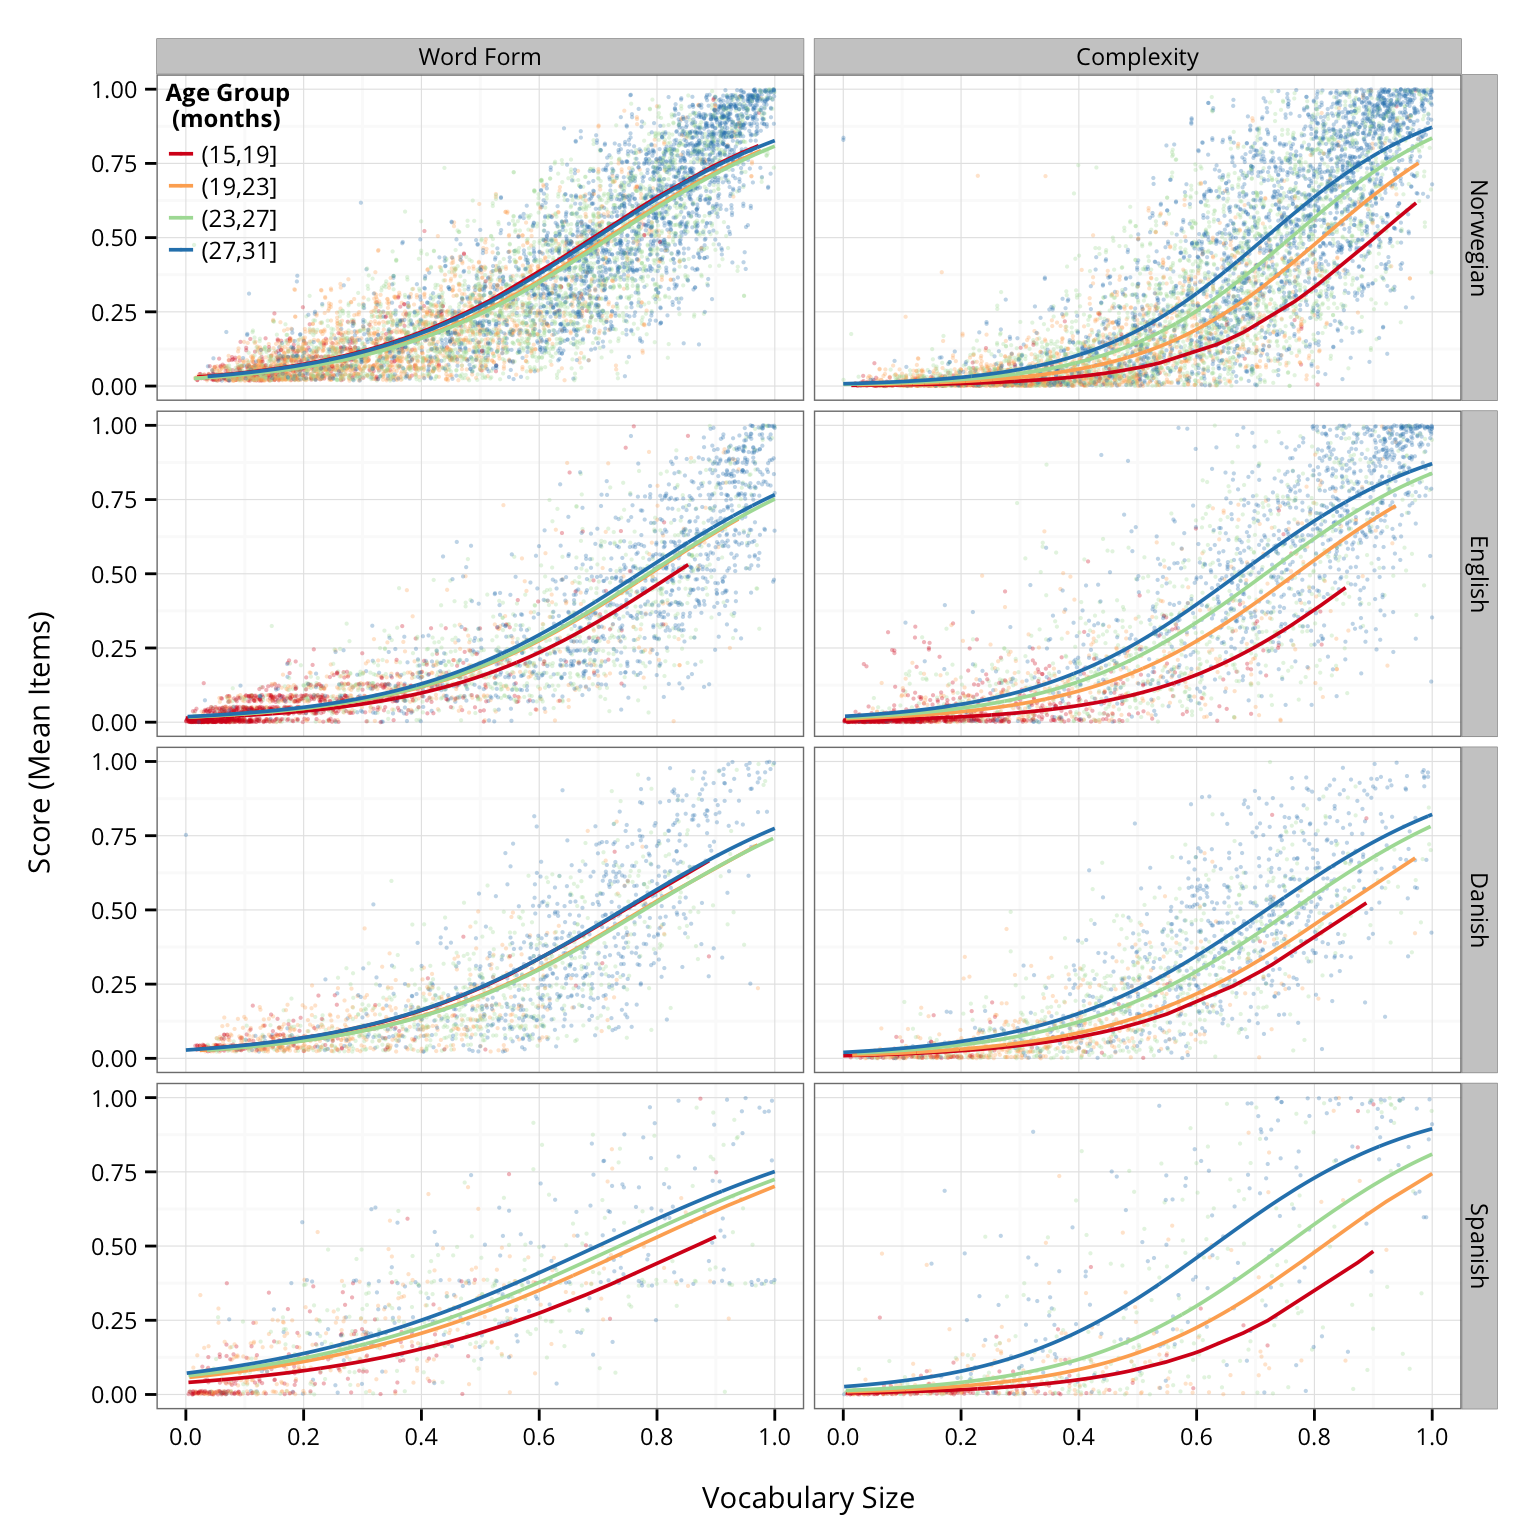
\includegraphics[width=.72\textwidth]{plots/grammar_data_plot-1.png}
\caption{\label{fig:grammar} Each point shows an individual child, indicating their total vocabulary size and Word Form or Complexity score, with color showing their age bin (English $n=4137$; Spanish $n=1094$; Norwegian $n=8505$; Danish $n=2074$). Panels show different languages, and curves are logistic regression models fit separately for each language and measure. The models were specified as {\small{\tt{score $\sim$ vocab + age}}}.} 
\end{figure*}

By two years, most children have a sizable working vocabulary, including verbs, prepositions, and closed class forms that perform grammatical work. They are also beginning to use multi-word combinations (e.g., \emph{mommy sock}) and may demonstrate productive use of inflectional morphemes (e.g., past tense \emph{-ed}). Previous studies have found a strong connection between the size of the lexicon and grammatical development as measured by the Complexity section, in many languages including English, Italian, Hebrew, and Spanish \cite<see>{bates1999}. However, no study has had the power and cross-linguistic representation to go beyond this initial finding to explore relations to grammatical items that vary in morphological/syntactic features. We extend this work by examining grammatical development using two measures: the Word Form checklist as a window into morphology and the Complexity checklist as a window into syntax. For each measure, we investigate the effects of vocabulary size and age.

%This suggests that the mechanisms guiding vocabulary and grammar learning are highly interdependent \cite{tomasello2003,bresnan2001}, a view at odds with the nativist assumption that grammar emerges independent of the lexicon \cite{chomsky1981}.

\subsubsection{Results}

\begin{figure}
\begin{center}
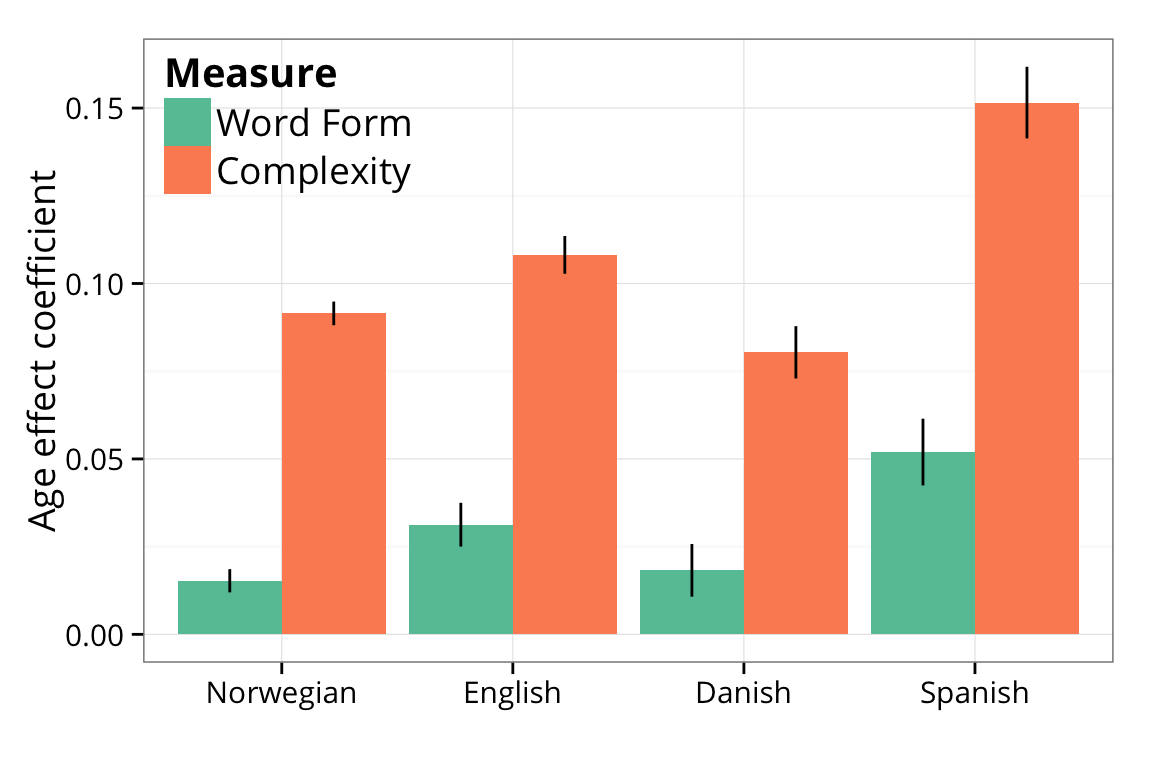
\includegraphics[width=\linewidth]{plots/grammar_coef_plot-1.png}
\end{center}
\caption{\label{fig:coefs_grammar} For each language and measure, the model's age effect coefficient. Ranges show the 95\% confidence interval of the coefficient estimate. Across languages, Complexity has a substantially larger age effect than Word Form.}
\end{figure}

\begin{figure}
\centering
\fbox{\parbox[b][][c]{7.3cm}{\centering All data and code for these analyses are available at\\ \url{https://github.com/dyurovsky/cdi-grammar}}}
\end{figure}

We wanted to estimate how much variance in children's syntactic and morphological development remains after accounting for that child's vocabulary size. Specifically, we asked whether age provides additional predictive power beyond vocabulary size. To estimate this effect, we fit logistic regression models to each child's Word Form and Complexity scores, predicting score as a function of vocabulary size and age in months. For all languages and measures, the evidence is overwhelmingly in favor of the model using both vocabulary and age as predictors, as compared to the model using only vocabulary (the smallest difference in AIC is 76). %Main effects were always exceedingly reliable, but the interaction term had negligible magnitude and so we omit it here.

Figure~\ref{fig:grammar} shows the data and models: each point represents a child's score on a measure, while curves show the relationship between score and vocabulary size.
%As seen most clearly for English and Norwegian---the languages for which we have most data---
For all languages, the curves for Word Form are nearly overlapping, showing little differentiation across age groups. This indicates only small contributions of age above and beyond vocabulary. In contrast, the curves for Complexity show a characteristic fan across age groups, indicating that the relationship between vocabulary size and complexity score is modulated by age. %The Spanish and Danish data show less of a clear complexity curve fan, possibly because of the relatively small number of data points in the youngest age group.

\begin{figure*}
\centering
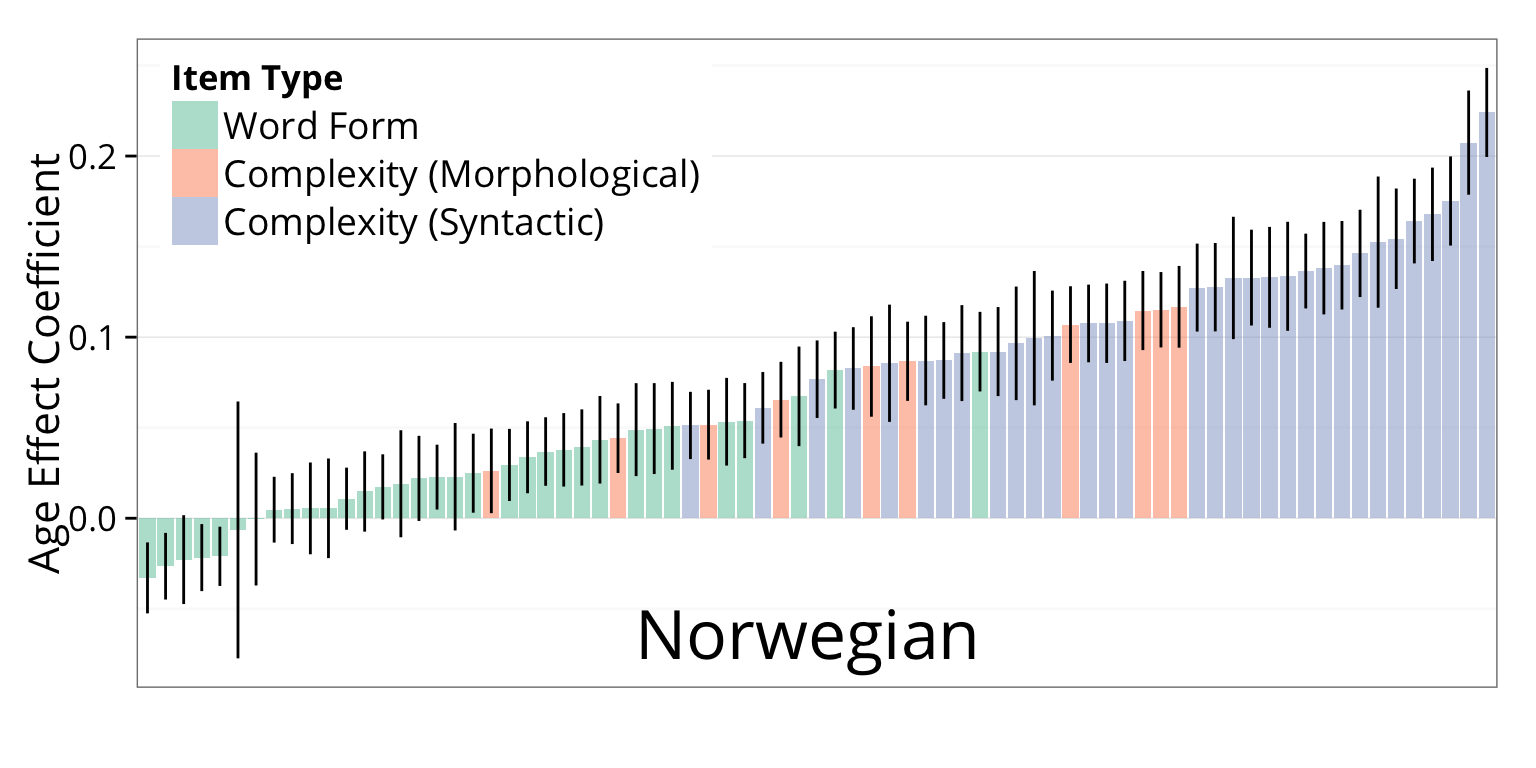
\includegraphics[width=.45\textwidth]{plots/item_coef_plot_norwegian-1.png}
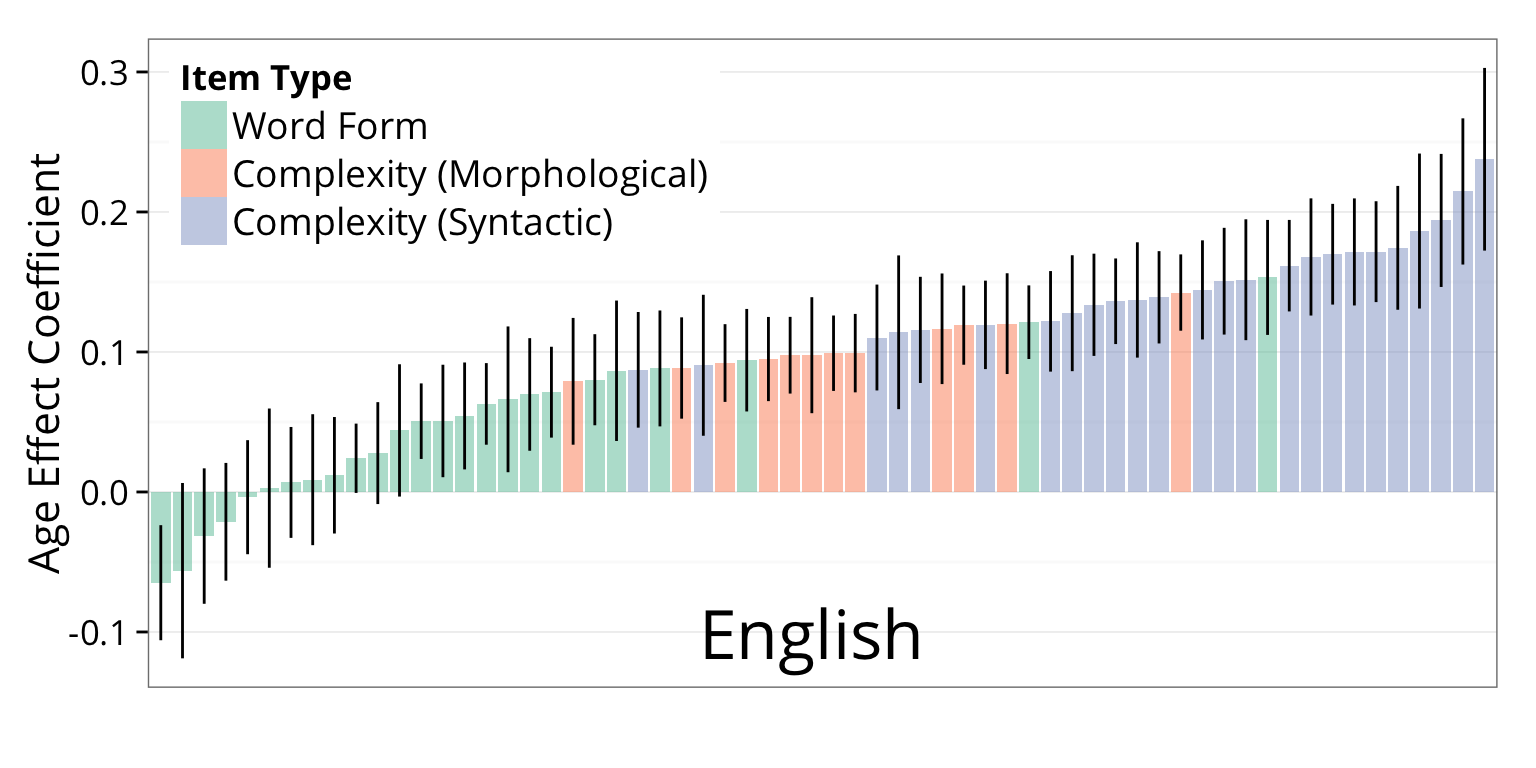
\includegraphics[width=.45\textwidth]{plots/item_coef_plot_english-1.png}\\
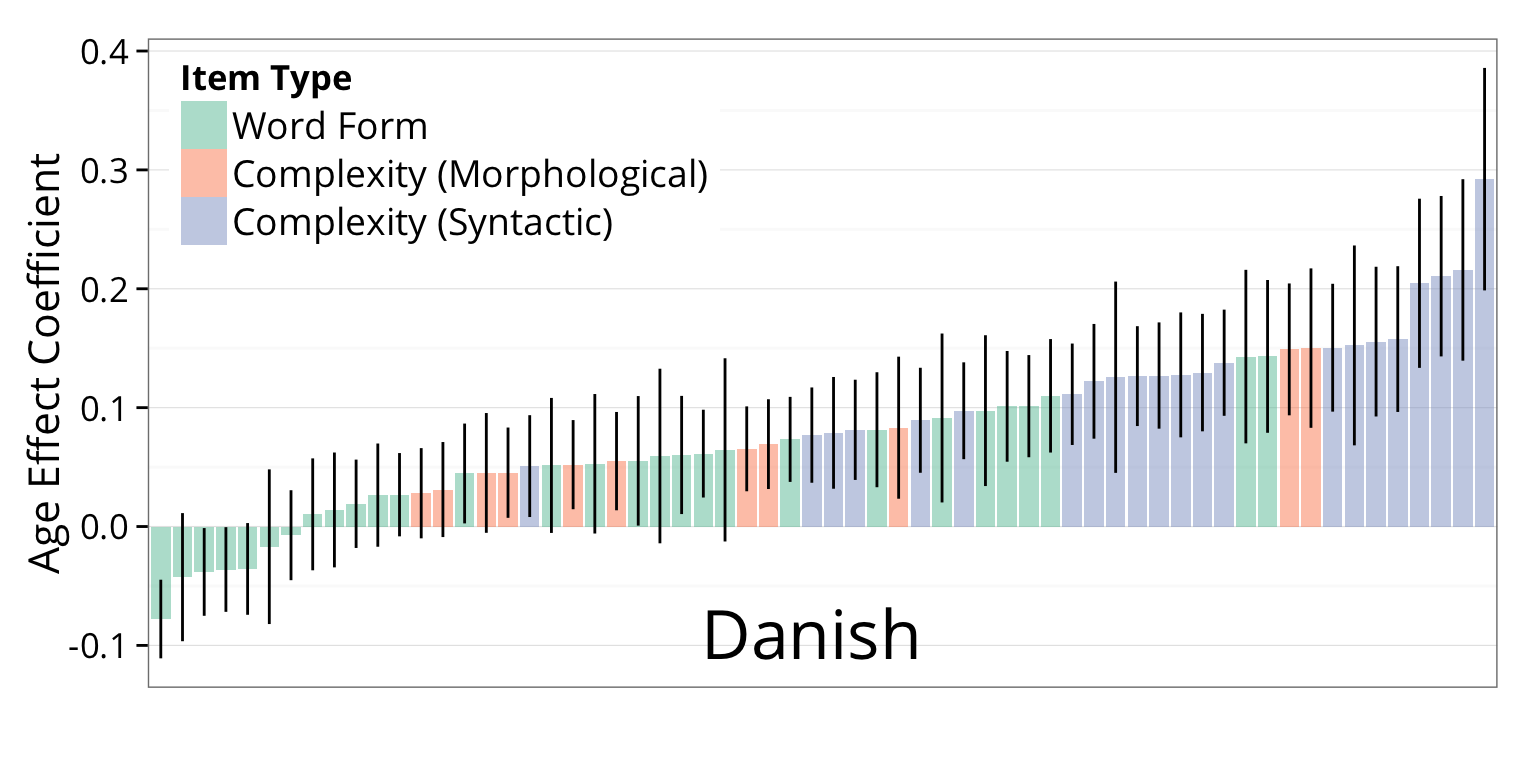
\includegraphics[width=.45\textwidth]{plots/item_coef_plot_danish-1.png}
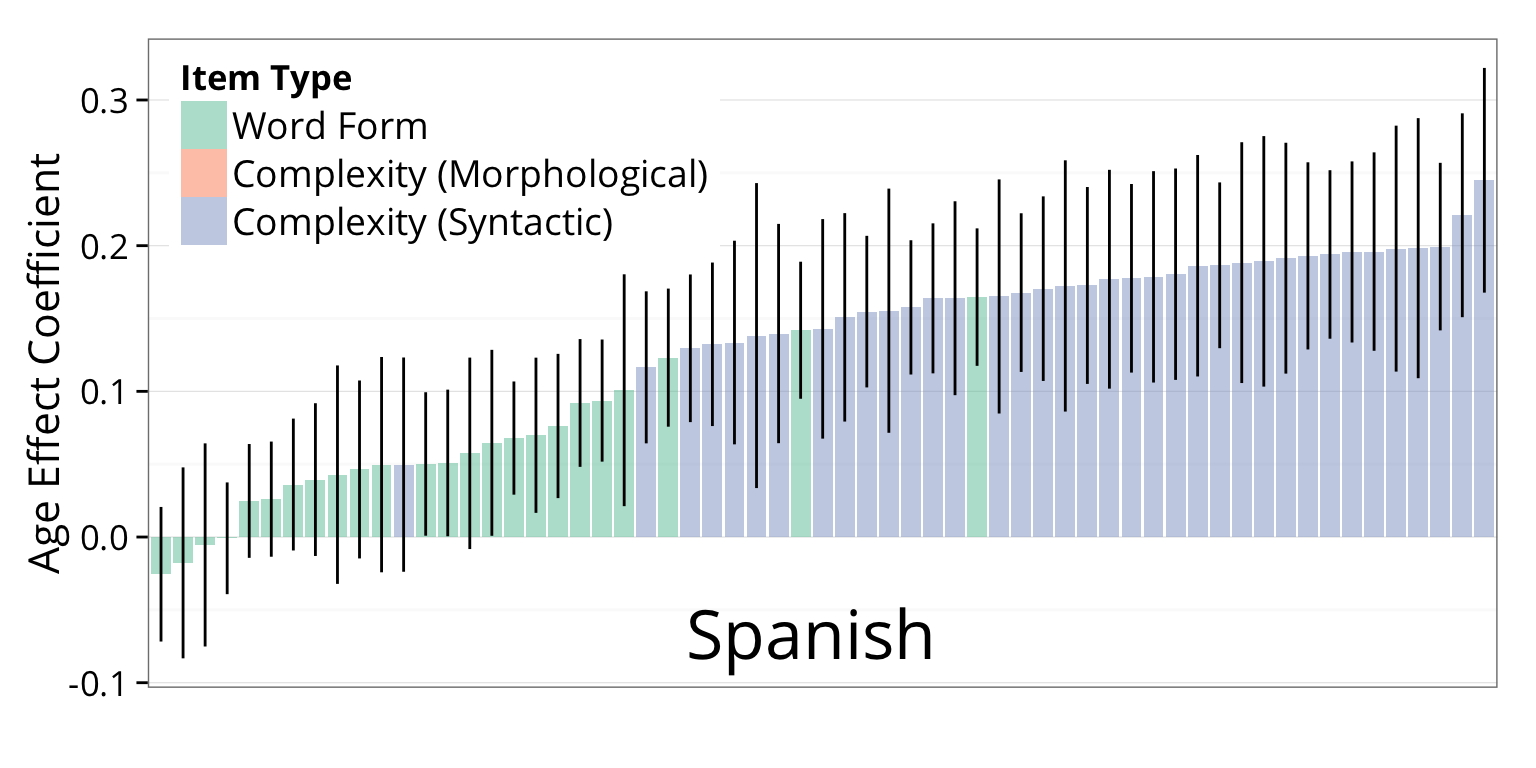
\includegraphics[width=.45\textwidth]{plots/item_coef_plot_spanish-1.png}
\caption{\label{fig:interactions} For each language and item, the model's age effect coefficient. Ranges show the 95\% confidence interval of the coefficient estimate. Across languages, Word Form items tend to have smaller age effects, Morphological Complexity items tend to have middling age effects, and Syntactic Complexity items tend to have larger age effects. (Note: No Spanish complexity items had exclusively morphological content.)}
\end{figure*}

Because of the size of our samples, all main effects and interactions are highly significant. To assess the extent of the age contribution to children's morphological and syntactic development, we compared the coefficients of Word Form and Complexity models. Figure~\ref{fig:coefs_grammar} shows the coefficient of the age effect for each measure across languages. In each language, the age effect coefficient is substantially larger for Complexity than for Word Form, indicating a greater age effect on those items that generally align with syntax than morphology.

Given the heterogeneous nature of the CDI instruments, particularly in the Complexity sections, we further broke down these items by classifying them as capturing more morphological or more syntactic phenomena. Items for which the difference between the simple and complex sentences is in the inflection of a noun or verb (such as \emph{doggie kiss me / doggie kissed me}) were coded as Morphological. The remainder of the items were coded as Syntactic, since they involve the use of some sentence-level syntactic construction (such as \emph{doggie table / doggie on table}).

We then fit predictive models as above separately for every item. Figure \ref{fig:interactions} shows the age effect coefficient for each item. In general, there is a three-way split: age effects are smallest for Word Form items, then Morphological Complexity items, and largest for Syntactic Complexity items, suggesting that more syntactic phenomena have greater age contributions. 

\vfill
\subsubsection{Discussion}

Building on previous analyses that showed a strong relationship between lexical and grammatical development, we incorporated age into this relationship. Across languages, our measures of syntactic development consistently showed greater age modulation than measures of morphological development. Further, distinguishing between items that were more reflective of syntax than morphology, we again found greater age effects for more syntactic items. Thus, this analysis provides evidence for a relationship between syntactic development and age \emph{not} captured by lexical development.

\subsection{Analysis 2: Vocabulary Composition}

Early vocabulary development is typically characterized by the learning of names for caregivers and common objects, while later in development, children tend to diversify their vocabulary by increasing the proportion of predicates (verbs and adjectives) and closed class words. This over-representation of nouns has been found across a number of analyses and in a variety of languages \cite{bates1994,caselli1995,bornstein2004}, though not all \cite{tardif1996,choi1995}.
%\footnote{Differences in early vocabulary composition have been argued to emerge from typological differences (e.g., word order, subject drop), and from cultural practices (e.g., focus on picture book reading) \cite{tardif1999, gopnik1996, choi1995}---we are agnostic as to the source of this variability.}
For our purposes, we are interested in using these analyses of vocabulary composition to test for the same kind of age-related differences that we found in the Complexity and Word Form analyses. 

\begin{figure*}
\begin{center}
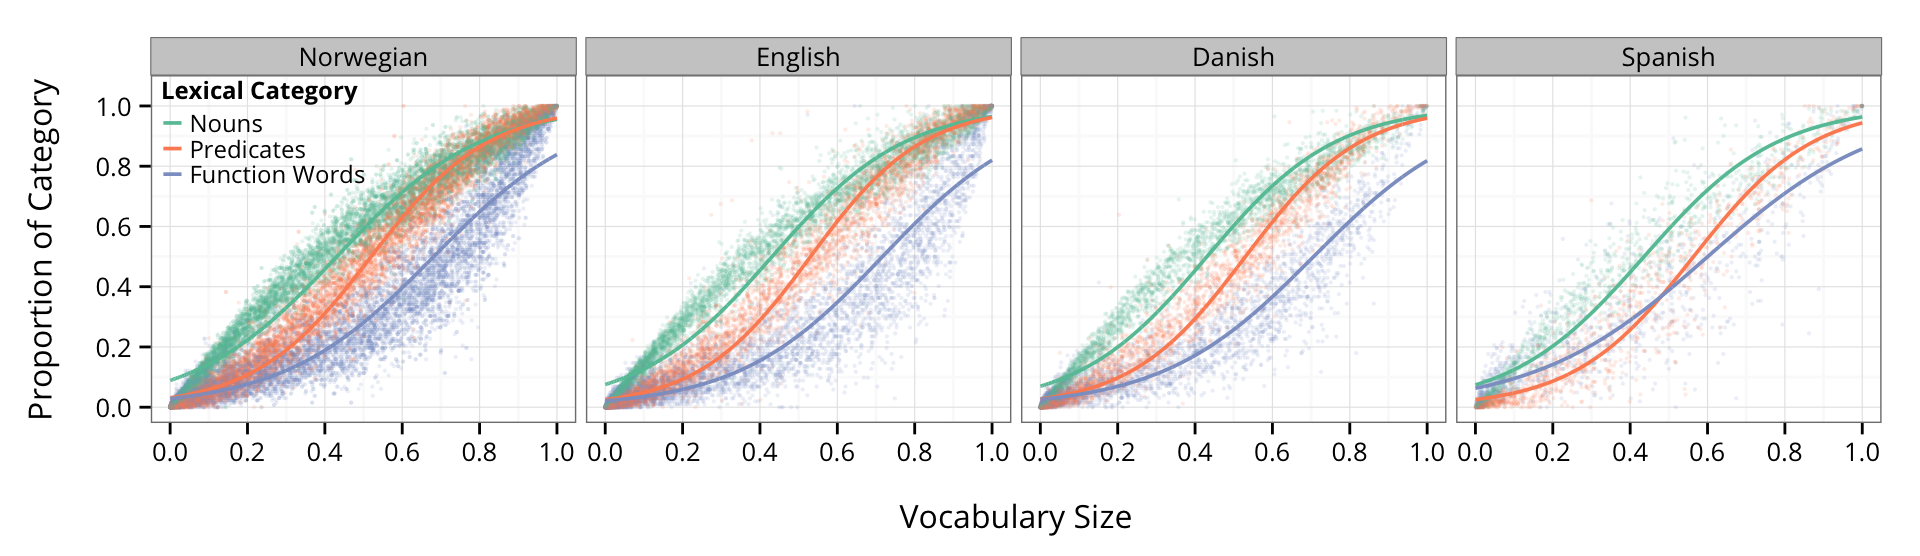
\includegraphics[width=\linewidth]{plots/vocab_data_plot-1.png}
\end{center}
\caption{\label{fig:vocab_comp} Proportion of a particular CDI category, plotted by total vocabulary size. Each point shows an individual child, with color showing their noun, predicate, and function word vocabulary. Panels show different languages, and curves are regression models fit separately for each language, specified as \small{\tt{proportion $\sim$ vocab + age}} (English $n=5595$; Spanish $n=1094$; Norwegian $n=10095$; Danish $n=3038$).}
\end{figure*}

We predict that age should have relatively more effect on the proportion of predicates and function words in children's vocabularies than on the proportion of nouns. Concrete nouns are hypothesized to be learned initially from both co-occurrences between words \cite{yu2007b} and by social cues to reference to particular objects \cite{bloom2002}. On neither account should syntactic information be a primary information source (though syntax might be more informative for abstract nouns). In contrast, for other types of words, syntax should be more important for learning their meaning.

On the syntactic bootstrapping hypothesis \cite{gleitman1990,fisher2010}, verbs especially are learned by mapping the syntactic structure of utterances to the thematic structure of observed events, for example by noticing that the subject of a sentence matches the agent in one particular ongoing event but not another (``the cat is fleeing the dog'' matches \textsc{flees(cat, dog)} but not \textsc{chases(dog, cat)}). A similar argument can be made for adjectives, since identification of the modified noun is similarly critical for inferring the meaning of the modifier. By the same logic, function words should be even harder to learn without some understanding of their syntactic relations. Thus, if syntactic development is related in some way to age, we should see larger age effects on predicate and function word acquisition than on noun acquisition. 

\subsubsection{Results}

Each CDI form contains a mixture of words in different classes. We adopt the categorization of \citeA{bates1994}, splitting words into nouns, predicates (verbs and adjectives), function words, and other words. For each child's vocabulary, we compute the proportion of the total words in each of these categories that they are reported to produce.

For each of the four languages in our sample, we plot these proportions against total vocabulary. These functions are shown in Figure \ref{fig:vocab_comp}: Each point represents a child's knowledge of a particular class, while curves show the relationship between a class and the whole vocabulary. If categories grow independently of one another, these curves should approximate the diagonal. This pattern is not what we observe, however: Across the languages in our sample, nouns are systematically over-represented in smaller vocabularies (shown by a curve that is above the diagonal), while function words---and to some extent, predicates---are under-represented. 

Next, we measure the contribution of age to vocabulary composition. We fit a logistic model to all children's data for each word class, predicting word-class proportion as a function of total vocabulary and age (as in Analysis 1). Figure \ref{fig:coefs_vocab_comp} shows age coefficients for each of these models across languages. In all four languages, the age coefficient is substantially larger for function words than for nouns. This asymmetry can be interpreted as evidence that, for two vocabulary-matched children, the older child would tend to produce relatively more function words than the younger. In English and Norwegian, the same regularity holds for predicates, while for Spanish and Danish, predicates and nouns are more similar to one another.

\subsubsection{Discussion}

We replicated previous analyses \cite{bates1994} showing an over-representation of nouns in the developing lexicon and an under-representation of predicates and function words. We also predicted that---if syntactic generalization was in some way tied to age---predicates and function words would show relatively more age influence than nouns. Although there was some cross-language variation in predicate terms, overall this prediction was confirmed across the languages we examined. Thus, this analysis provides additional evidence for a relationship between syntactic development and age, independent of the growth of the lexicon.

\begin{figure}
\centering
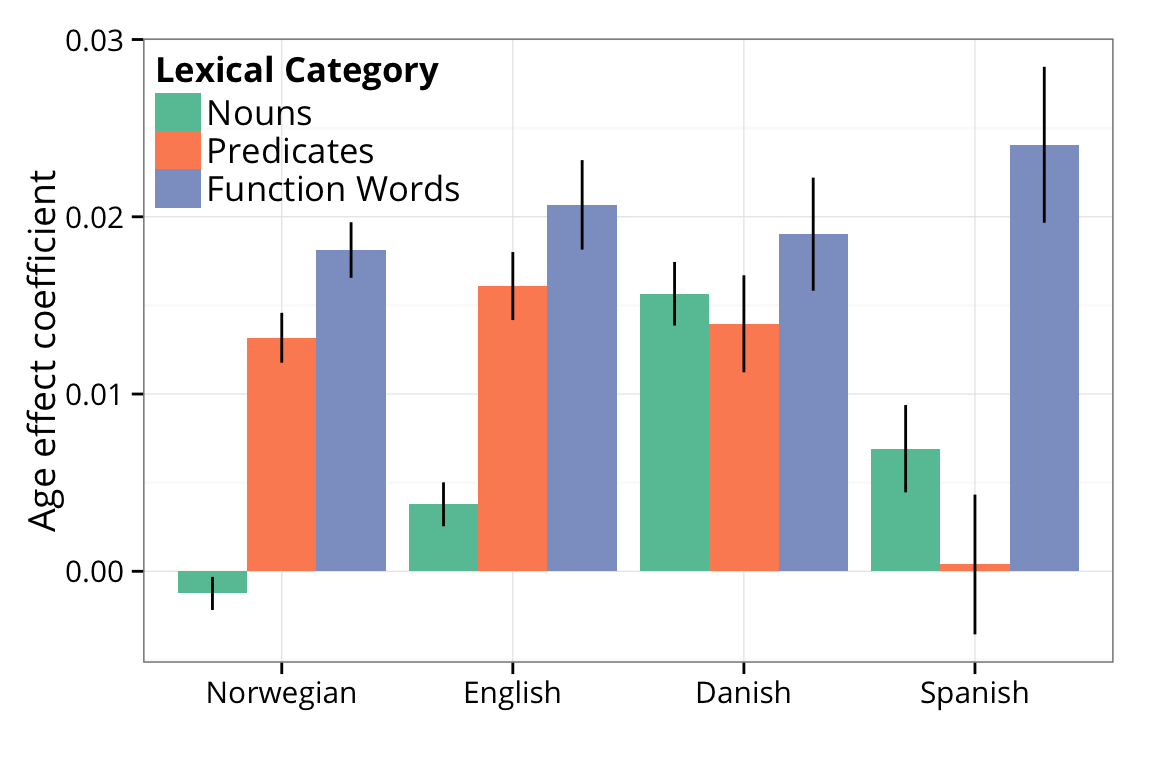
\includegraphics[width=\linewidth]{plots/vocab_coef_plot-1.png}
\caption{\label{fig:coefs_vocab_comp} For each language and lexical category, the model's age effect coefficient. Ranges show the 95\% confidence interval of the coefficient estimate. Across languages, predicates and function words tend to have a substantially larger age effect than nouns.}
\end{figure}

\section{General Discussion}

The current study revisits classic findings but also explores novel questions regarding lexicon-grammar relations and vocabulary composition through Wordbank, a newly-developed web-based tool for cross-linguistic analyses of large CDI datasets. Our results provided general support for a lexicalist view, in that, in four languages, variance in vocabulary production strongly aligned with variance in grammar. However, we also estimated additional age-related contributions, specifically contrasting the links to morphological forms vs. syntactic constructions, and to different lexical categories. In general, we find that measures of grammar that are more closely aligned with syntax are modulated by age to a greater extent than those reflecting morphology. Also, we find that the trajectories of predicate and function word representation in the vocabulary are modulated by age to a greater extent than noun representation (albeit with some variability across languages). Both findings suggest a place for developmental processes that facilitate grammatical acquisition beyond pure lexical growth.

Our analyses suggest interesting new areas of research regarding possible mechanisms driving children's early lexical development and how those mechanisms might support children's transition from single words to more grammatically complex utterances. One possibility is that these developments are dependent on maturational factors that operate on grammatical development in a domain-specific way, independent of lexical-semantic processes. Another possibility is that age-related effects represent more domain-general learning mechanisms, such as attention or working memory, that provide differential support for sentence-level processes than word-internal ones \cite{gathercole2014}. Future studies should also explore the extent to which lexical and age-related processes are shaped, either independently or in tandem, by features of the learning environments that children experience \cite<e.g.,>{weisleder2013}.

Questions about the nature of grammatical representations in early language have often seemed deadlocked. But by mapping out developmental change across large samples and multiple languages, our findings here challenge theories across the full range of perspectives to more fully describe the mechanistic factors underlying the interaction of vocabulary, grammar, and development. 

 % will require large-scale, cross-linguistic data of the type presented here. The use of richer, more detailed data allows the identification of 

% processing speed, working memory?

\section{Acknowledgments}

Thanks to the MacArthur-Bates CDI Advisory Board, Dorthe Bleses, Kristian Kristoffersen, Rune N\o rgaard J\o rgensen, and the members of the Language and Cognition Lab. 

\bibliographystyle{apacite}

\setlength{\bibleftmargin}{.125in}
\setlength{\bibindent}{-\bibleftmargin}

\bibliography{CogSci}

\end{document}
